\section{Experimental Results}


\subsection{Roadmap}
Our experiments try to answer the following questions:

\begin{itemize}
\item bla
\item bla2
\item bla3
\end{itemize}




\subsection{Compare to Oracle}


\subsection{Analysis}

\begin{figure*}[!t]
\centering
\subfloat[][Model size]{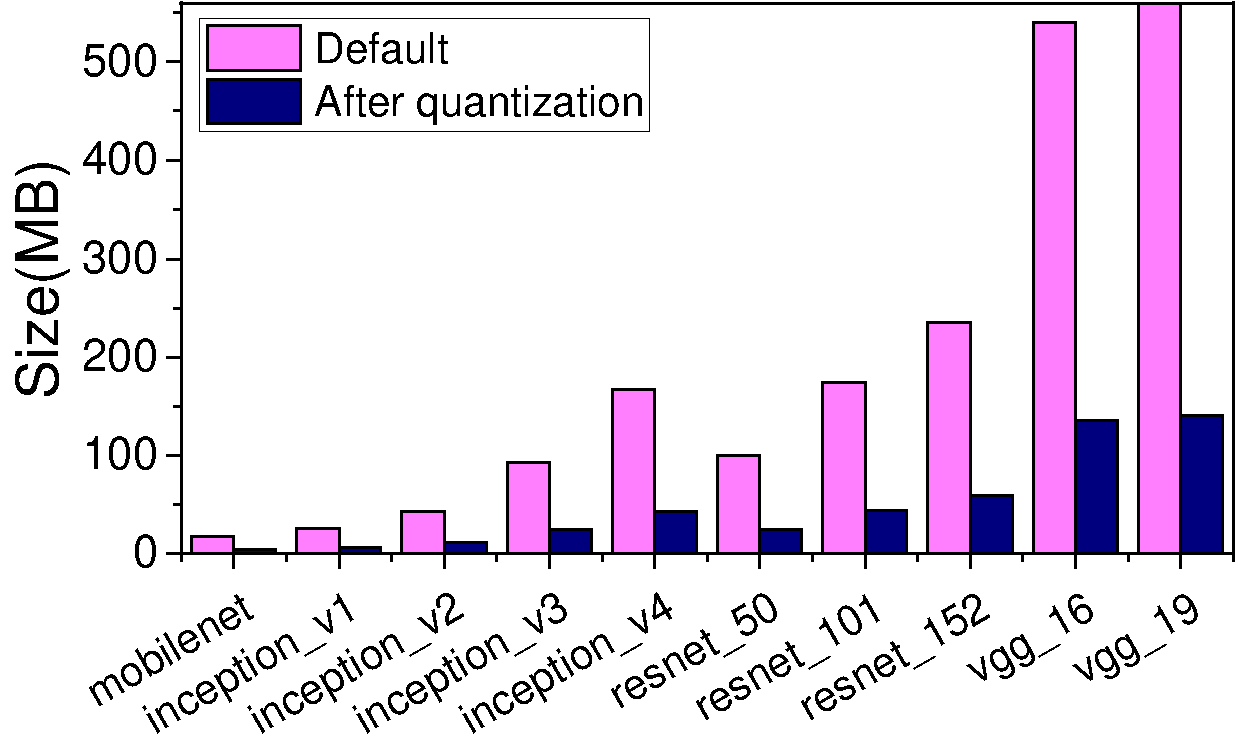
\includegraphics[width=0.3\textwidth]{figure/quan_size.pdf}}
\hfill
\subfloat[][Inference time]{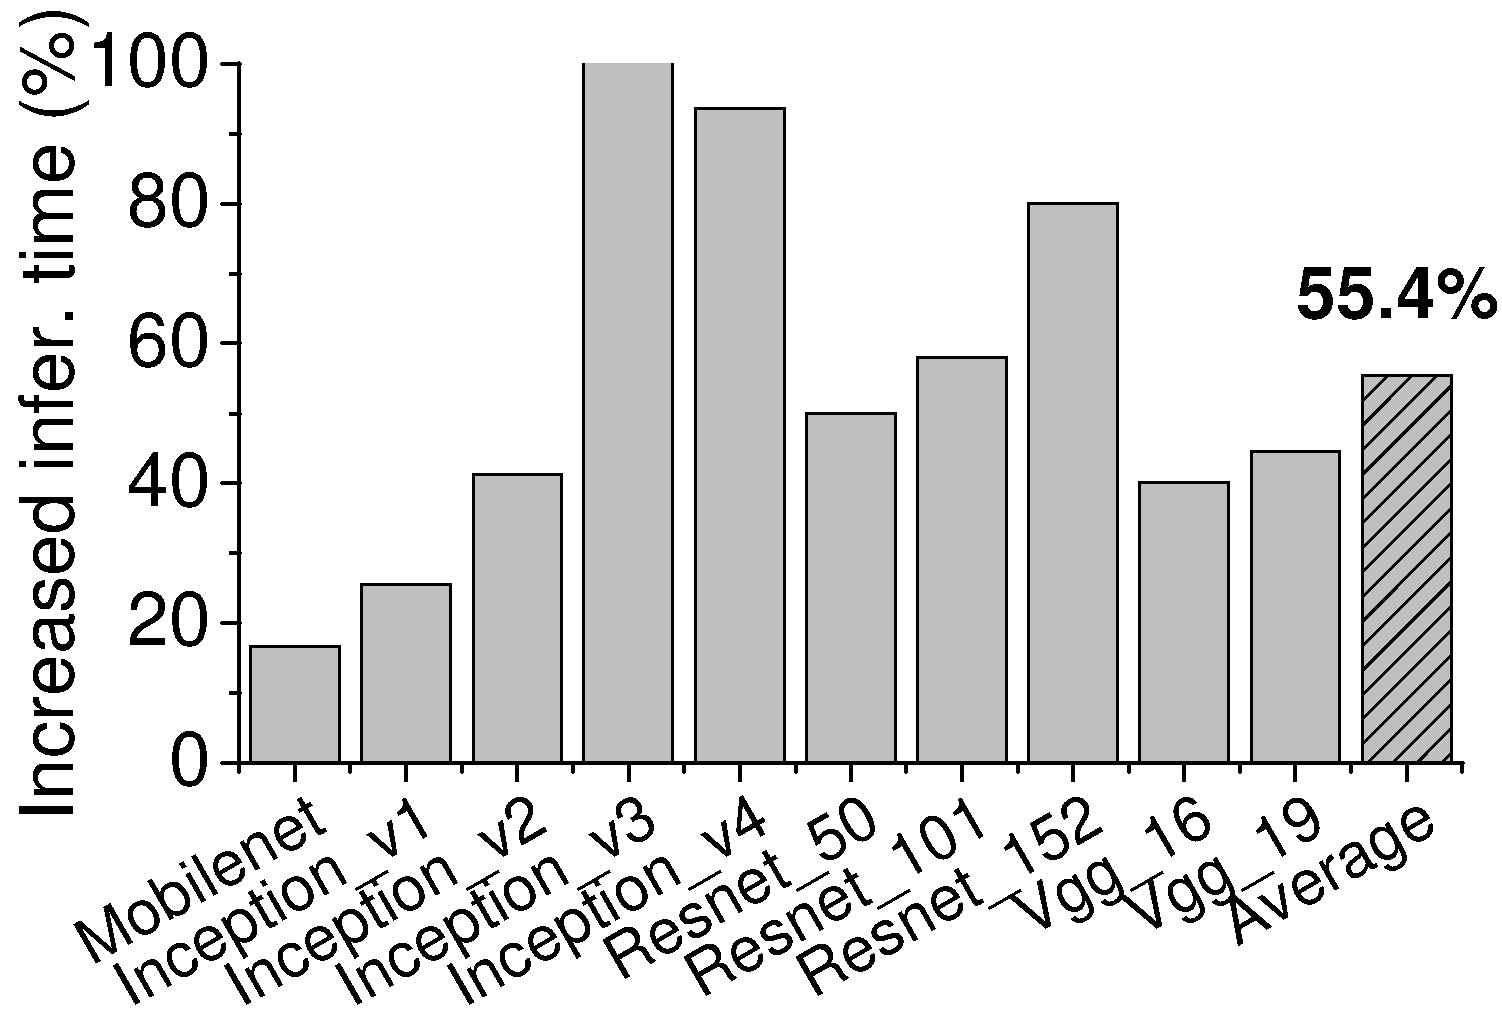
\includegraphics[width=0.3\textwidth]{figure/quan_time.pdf}}
\hfill
\subfloat[][Accuracy]{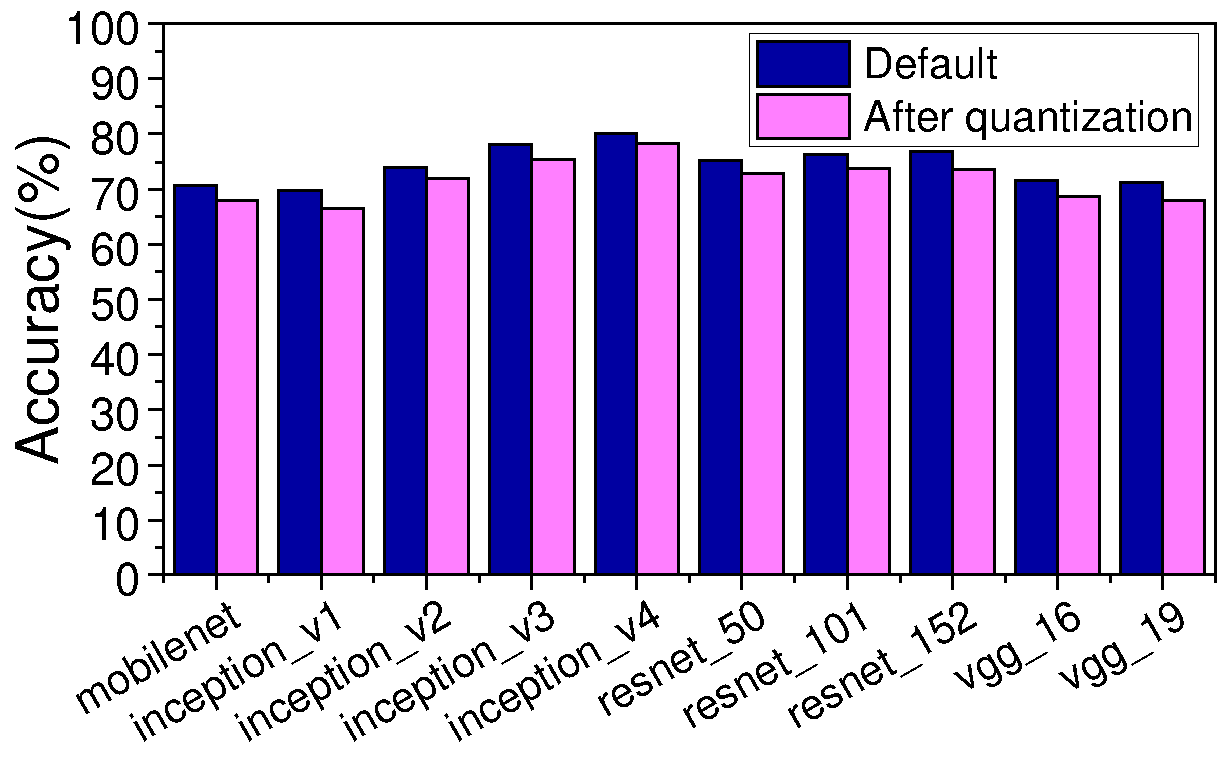
\includegraphics[width=0.3\textwidth]{figure/quan_acc.pdf}}
\hfill
\subfloat[][Power consumption]{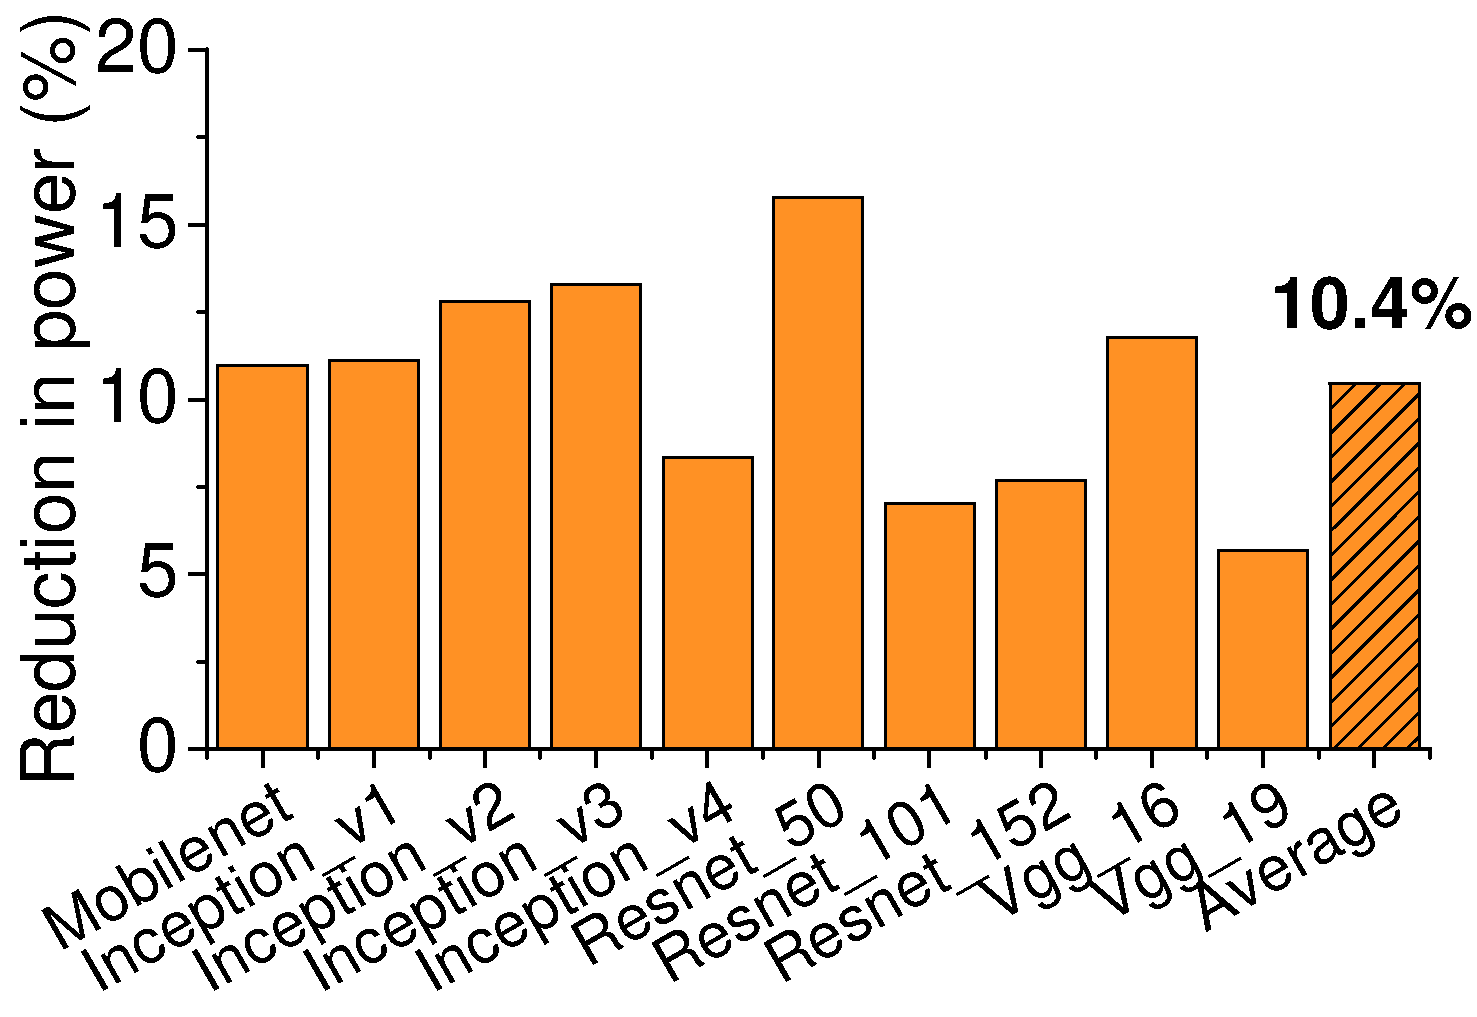
\includegraphics[width=0.4 	\textwidth]{figure/quan_power.pdf}}
\hfill
\subfloat[][Energy consumption]{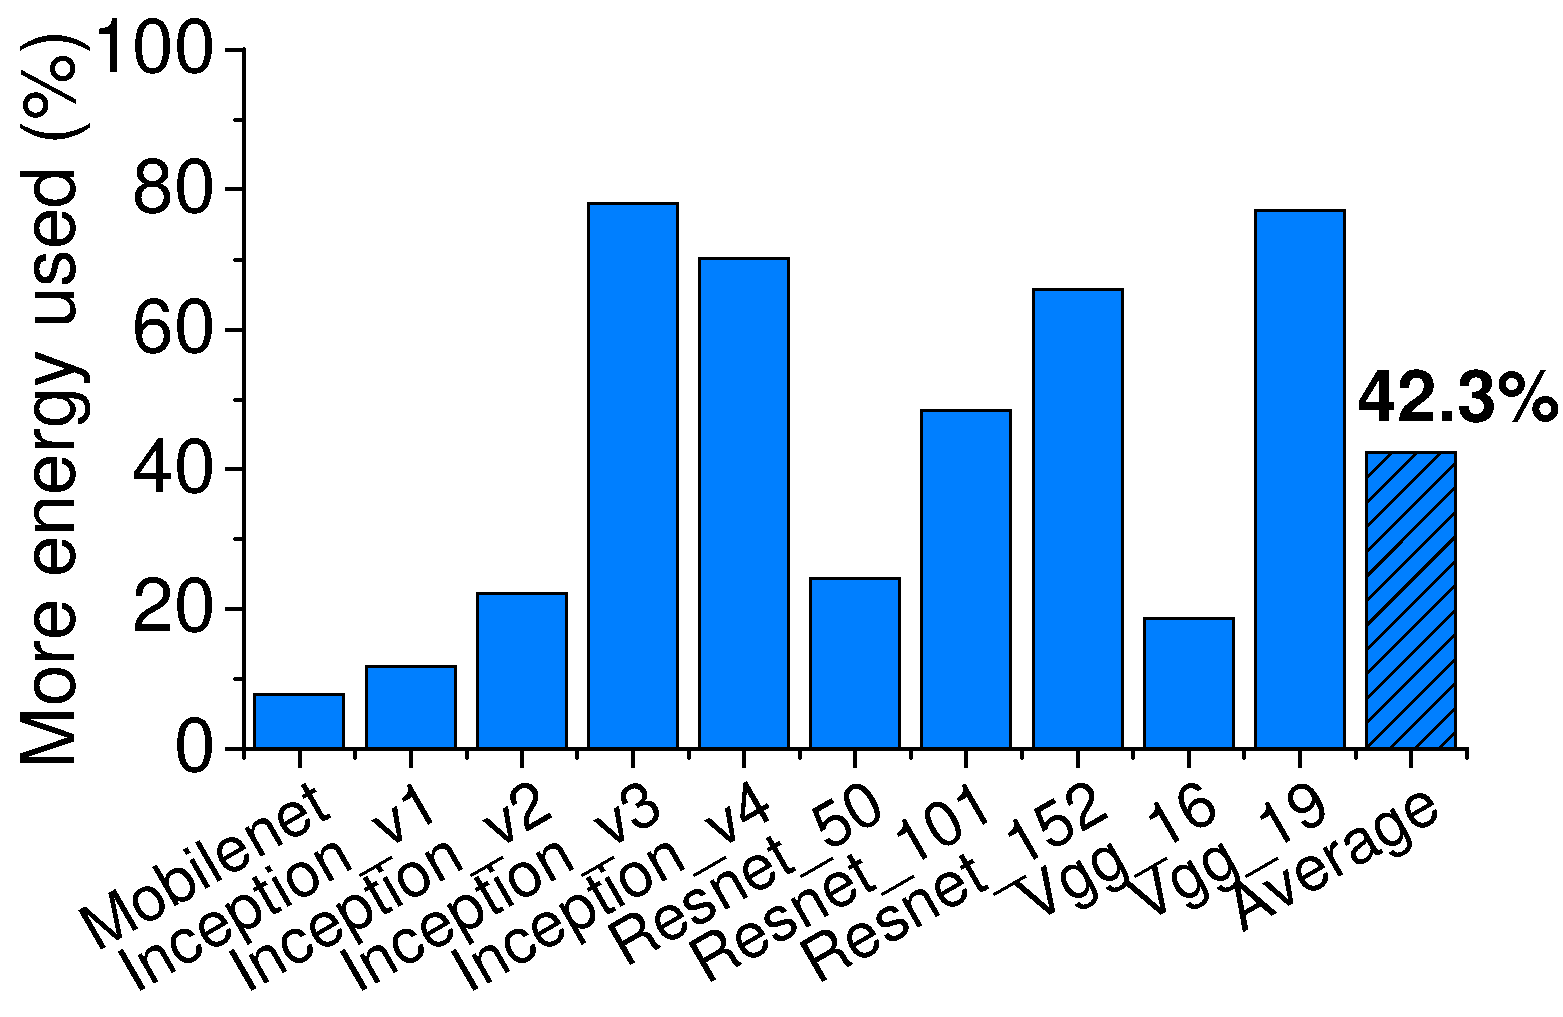
\includegraphics[width=0.4\textwidth]{figure/quan_energy.pdf}}
\hfill

\caption{The achieved model size (a) inference time (b) energy consumption (c) and accuracy (d) before and after the compression by \quantization and \pruning.
The compression technique to use depends on the optimization target.\FIXME{do something later}}
\label{fig:analy_quan}
\end{figure*}


\begin{figure*}[!t]
\centering
\subfloat[][Model size]{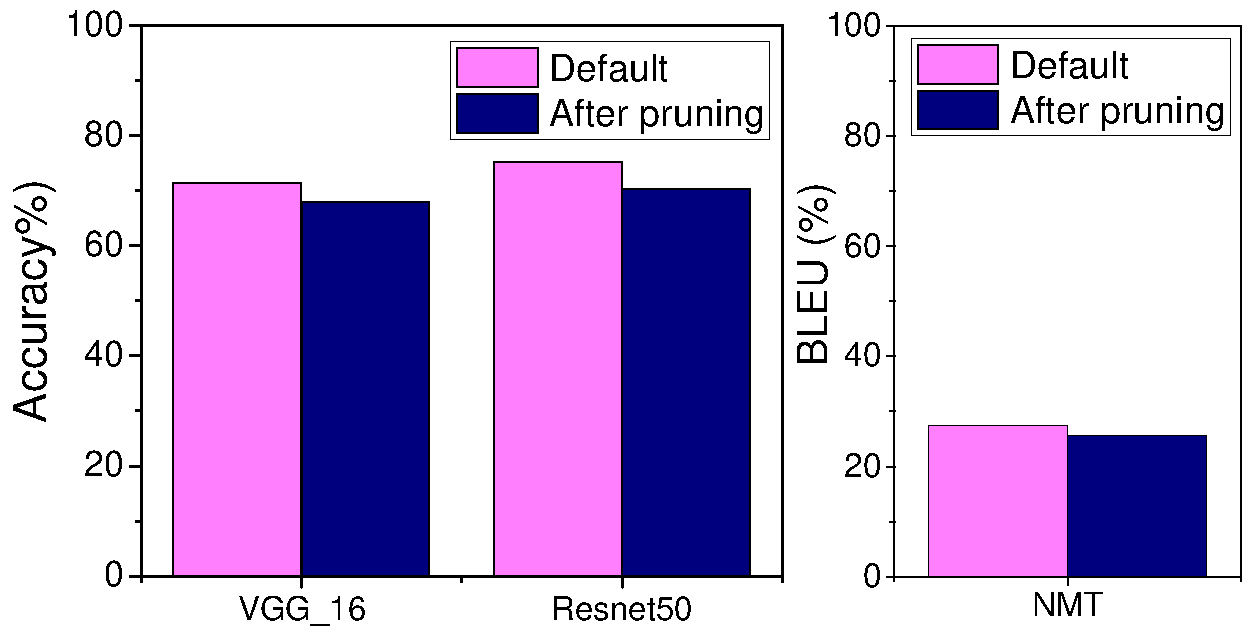
\includegraphics[width=0.4\textwidth]{figure/prun_acc.pdf}}
\hfill


\caption{The achieved model size (a) inference time (b) energy consumption (c) and accuracy (d) before and after the compression by \quantization and \pruning.
The compression technique to use depends on the optimization target.}
\label{fig:motivation}
\end{figure*}